\RequirePackage{fix-cm}
\documentclass[12pt]{article}

\usepackage{fixltx2e}
\usepackage[xetex]{graphicx}
\usepackage[nottoc,section]{tocbibind}
\usepackage[xetex,bookmarks]{hyperref}
\usepackage{bookmark}
\usepackage{xltxtra}
\usepackage[paper=letterpaper, margin=1in]{geometry}
\usepackage{layout}
\usepackage{multicol}
\usepackage{wrapfig}
\usepackage{calc}
\usepackage{etoolbox}
\usepackage{ccicons}
\usepackage[shortcuts]{extdash}
\usepackage{titling}
\usepackage[nodayofweek,24hr]{datetime}
\usepackage[monochrome,table]{xcolor}
\usepackage{environ}
\usepackage{longtable}
\usepackage{epsfig}
\usepackage[sectionbib,sort,numbers]{natbib}
\usepackage[shortlabels]{enumitem}
\usepackage{float}
\usepackage{wrapfig}
\usepackage{lettrine}

\newfontfamily\startrek{FederationClassic}
\newfontfamily\fatefont{Fate Core Glyphs}
\newfontfamily\handwritingfont[Scale=0.9]{Permanent Marker}

\setmainfont[Ligatures={Common,TeX}, Numbers={Proportional}]{Linux Libertine O}
\setmonofont[Scale=0.9]{Luxi Mono}

\urlstyle{same}

\renewcommand{\dateseparator}{-}

\newdateformat{mydate}{%
    \ifshowdow\dayofweekname{\THEDAY}{\THEMONTH}{\THEYEAR}\fi
    \THEDAY{} \monthname[\THEMONTH{}] \THEYEAR{}%
}

\makeatletter
\long\def\@makefntext#1{%
    \parindent 1em\noindent\hb@xt@ 1.8em{\hss\@makefnmark}~#1%
}
\makeatother

\newcommand{\STFLogo}{%
    {\startrek STAR} {\startrek TREK}:
    
\includegraphics[height=1em]{img/FateLightBW.pdf}%
}

\newcommand{\FateCore}{\textit{Fate Core}}
\newcommand{\StarTrek}{\textit{Star Trek}}
\newcommand{\StarTrekFate}{\textit{Star Trek: Fate}}

\newcommand{\skill}[1]{#1}
\newcommand{\aspect}[1]{\textbf{\textit{#1}}}
\newcommand{\stunt}[1]{\textbf{#1}}

\newcommand{\Ship}[1]{\textit{#1}}

\newcommand{\Class}[1]{\Ship{#1}\-/class}

\newenvironment{example}[0]{%
    \begin{quotation}\noindent\itshape\textbf{Example:}%
}{%
    \end{quotation}%
}

\newcommand{\AdjWord}[1]{%
    \ifnumequal{#1}{-2}{Terrible}{}%
    \ifnumequal{#1}{-1}{Poor}{}%
    \ifnumequal{#1}{0}{Mediocre}{}%
    \ifnumequal{#1}{1}{Average}{}%
    \ifnumequal{#1}{2}{Fair}{}%
    \ifnumequal{#1}{3}{Good}{}%
    \ifnumequal{#1}{4}{Great}{}%
    \ifnumequal{#1}{5}{Superb}{}%
    \ifnumequal{#1}{6}{Fantastic}{}%
    \ifnumequal{#1}{7}{Epic}{}%
    \ifnumequal{#1}{8}{Legendary}{}%
}

\newcommand{\SignedNumber}[1]{%
    \ifnumcomp{#1}{>}{-1}{+}{}#1%
}

\newcommand{\AdjLevel}[1]{%
    \AdjWord{#1} (\SignedNumber{#1})%
}

\newcommand{\SkillActionName}[1]{%
    \ifstrequal{#1}{O}{Overcome}{}%
    \ifstrequal{#1}{C}{Create an Advantage}{}%
    \ifstrequal{#1}{A}{Attack}{}%
    \ifstrequal{#1}{D}{Defend}{}%
}

\newlength{\currentparindent}
\NewEnviron{SkillActionList}{%
    \setlength{\currentparindent}{\parindent}%
    \begin{longtable}[l]{p{25pt}p{\linewidth-45pt}}%
        \BODY%
    \end{longtable}%
    \vspace*{-1em}%
}

\newcommand{\SkillActionEntry}[2]{%
    \raisebox{-10pt}{\Huge\fatefont{}{#1}}&%
    \setlength{\parindent}{\currentparindent}%
    \noindent\textbf{{\SkillActionName{#1}:}} #2 \\ & \\%
}

\newcommand{\skillitem}[1]{%
    \item[{\raisebox{-10pt}[0pt][0pt]{\Huge\fatefont{}{#1}\vspace{10pt}}}]%
}

%\newlength{\currentparindent}
\NewEnviron{SkillAction}[1]{%
    \noindent%
    \setlength{\currentparindent}{\parindent}%
    \parbox[t]{7ex}{\vskip0pt\Huge\fatefont {#1}}%
    \hfill%
    \parbox[t]{\linewidth-7ex}{%
        \vskip0pt%
        \setlength{\parindent}{\currentparindent}%
        \noindent\textbf{{\SkillActionName{#1}}:}
        \BODY%
    }%
}

\newlength{\SkillBoxWidth}
\setlength{\SkillBoxWidth}{6.2em}
\newcommand{\SkillBox}[1]{%
\framebox{\parbox[c][1em][c]{\SkillBoxWidth}{\centering\upshape\handwritingfont #1}}%
    \hspace{3pt}%
}

\newcommand{\blankpage}{%
    \newpage%
    \thispagestyle{empty}%
    \mbox{}%
    \newpage%
}



\title{Our \STFLogo{} Setting}
\author{Chris Bouchard}
\date{\mydate\today}

\begin{document}

\maketitle

Welcome to this game of \StarTrekFate{}. This document will describe the
setting in which our game takes place.

\section{Time Period}
Our game takes place in the year 2315, stardate 3574.5, in a Federation
controlled sector of the Alpha Quadrant. For perspective, the events of the
original series took place between 2265 and 2269, and Next Generation between
2364 and 2370. Friendly relations with the Klingon Empire were quite recently
established in 2293. The Federation is entering into the first extended period
of peace it has seen in a while.

Starfleet has begun phasing in a new style of uniform --- the familiar uniforms
of the Next Generation series\footnote{We will be using the Next Generation
uniforms with collars, which were used from the second season onward. The
collarless uniforms from the first season were just ugly and likely a budgetary
decision.} --- and with them the new \emph{combadges}. Some older officers
still reach for their communicator out of habit, but cadets graduating the
Academy these days may only have used a hand-communicator in training
exercises.

\begin{wrapfigure}{r}{0.4\linewidth}
    \centering
    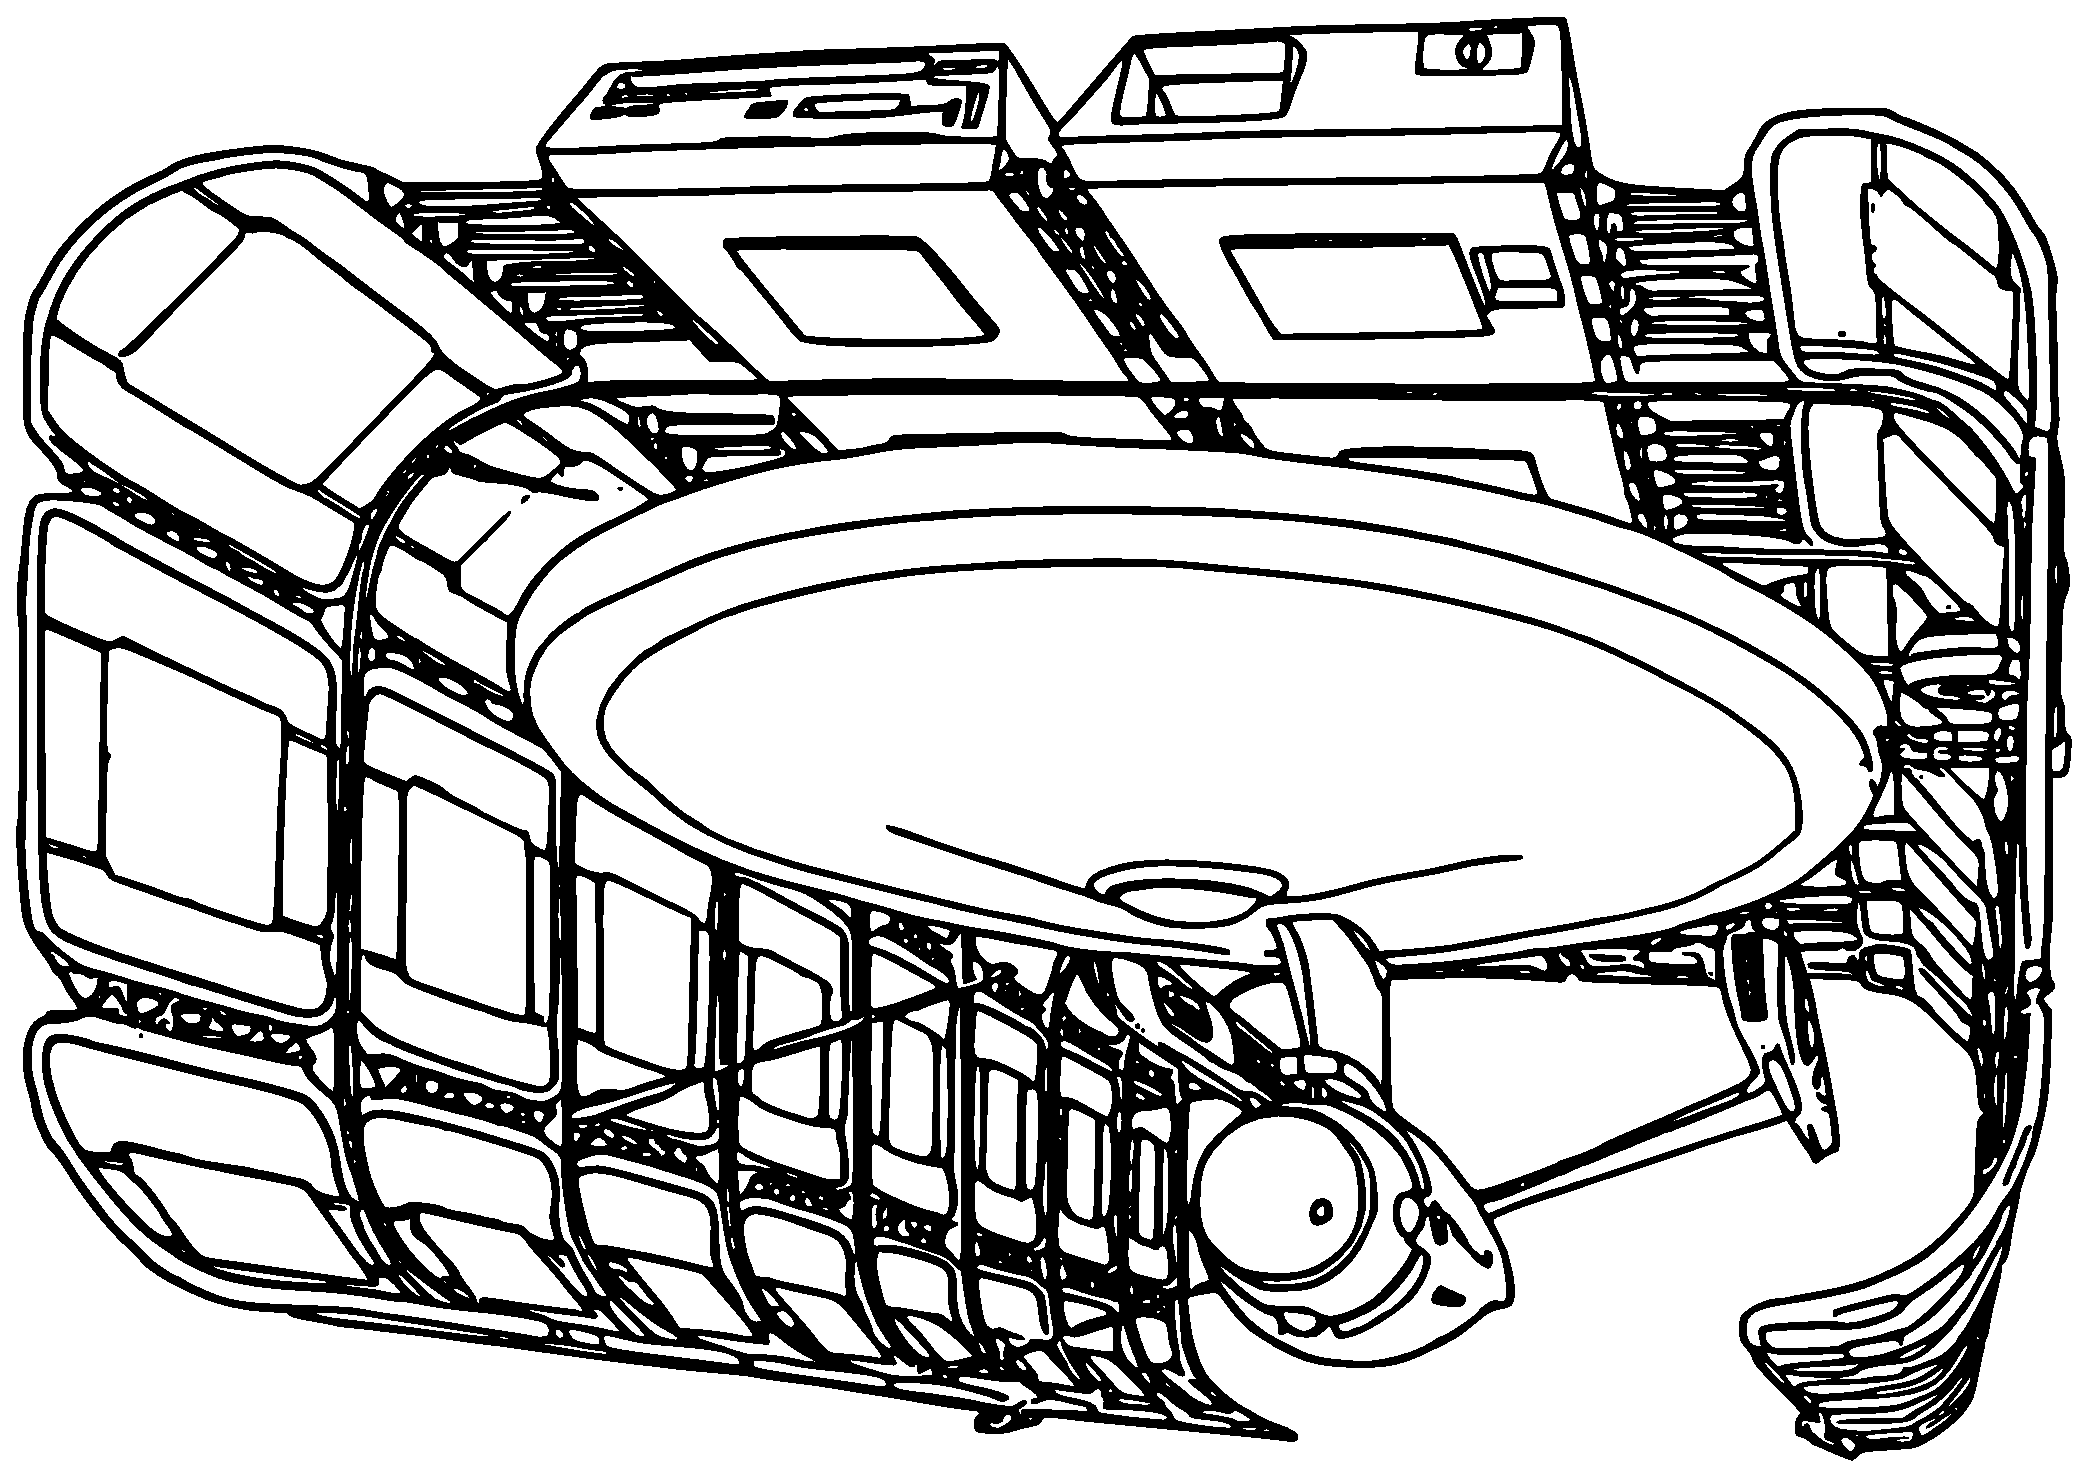
\includegraphics[width=0.8\linewidth]{img/SpaceDock.eps}\\
    \vspace{2ex}
    \footnotesize A newly-built ship in spacedock
    \vspace{-2em}
\end{wrapfigure}

The type two phaser is still the standard strength, but Starfleet is
replacing the old pistol-style phasors with a newer, sleeker design to
emphasize phasers as tools rather than weapons. Both are in service at the
moment, though any newly issued phaser will be the new style.

\section{What is Happening}
The first session will take place aboard a Federation space station, where the
crew of a newly commissioned \Class{Excelsior} starship will meet and take
their stations. Each of your characters has been selected by Starfleet for this
post --- definitely an honor.

Where we go from here is up to you. During character creation you will, as a
group, pick two issues that you want to tackle in this game. I will use those
and your character backstories to build a story that everyone will enjoy.
During the first session of play, you will receive your first mission from
Starfleet Command.

\section{Major Players}
The biggest player is certainly The United Federation of Planets. It spans two
quadrants and is composed of over a hundered formal member worlds and over a
thousand colonies. Member planets are largely autonomous and have their own
local laws, with the Federation playing a similar role to the European Union of
21st century Earth.

Thanks to the actions of the \Ship{USS Excelsior} and \Ship{USS Enterprise-A}
during the Praxis crisis only twenty years ago, the Federation has found a new
ally in the Klingon Empire, though many on both sides remain skeptical of the
alliance. The Klingon way of life is still foreign to most in the Federation,
who view the Klingons as a bunch of savages. Rebellious teenagers listen to
Klingon ``music'' to annoy their parents.

The cold war with the Romulan Star Empire drags on. Ships still patrol the edge
of the neutral zone, and each side is looking for any new technology to gain an
advantage over the other. There has not, however, been much in the way of open
conflict.

Lately the Cardassian Union is an increasing threat to peace in the Alpha
Quadrant. Though the Cardassians have not attacked the Federation directly,
their militaristic and imperialistic policies are causing tension with the
Federation's new Klingon allies. Federation-Cardassian relations are still in
the earliest stages, and not much is known about their culture or customs.

\begin{wrapfigure}{l}{0.45\linewidth}
    \centering
    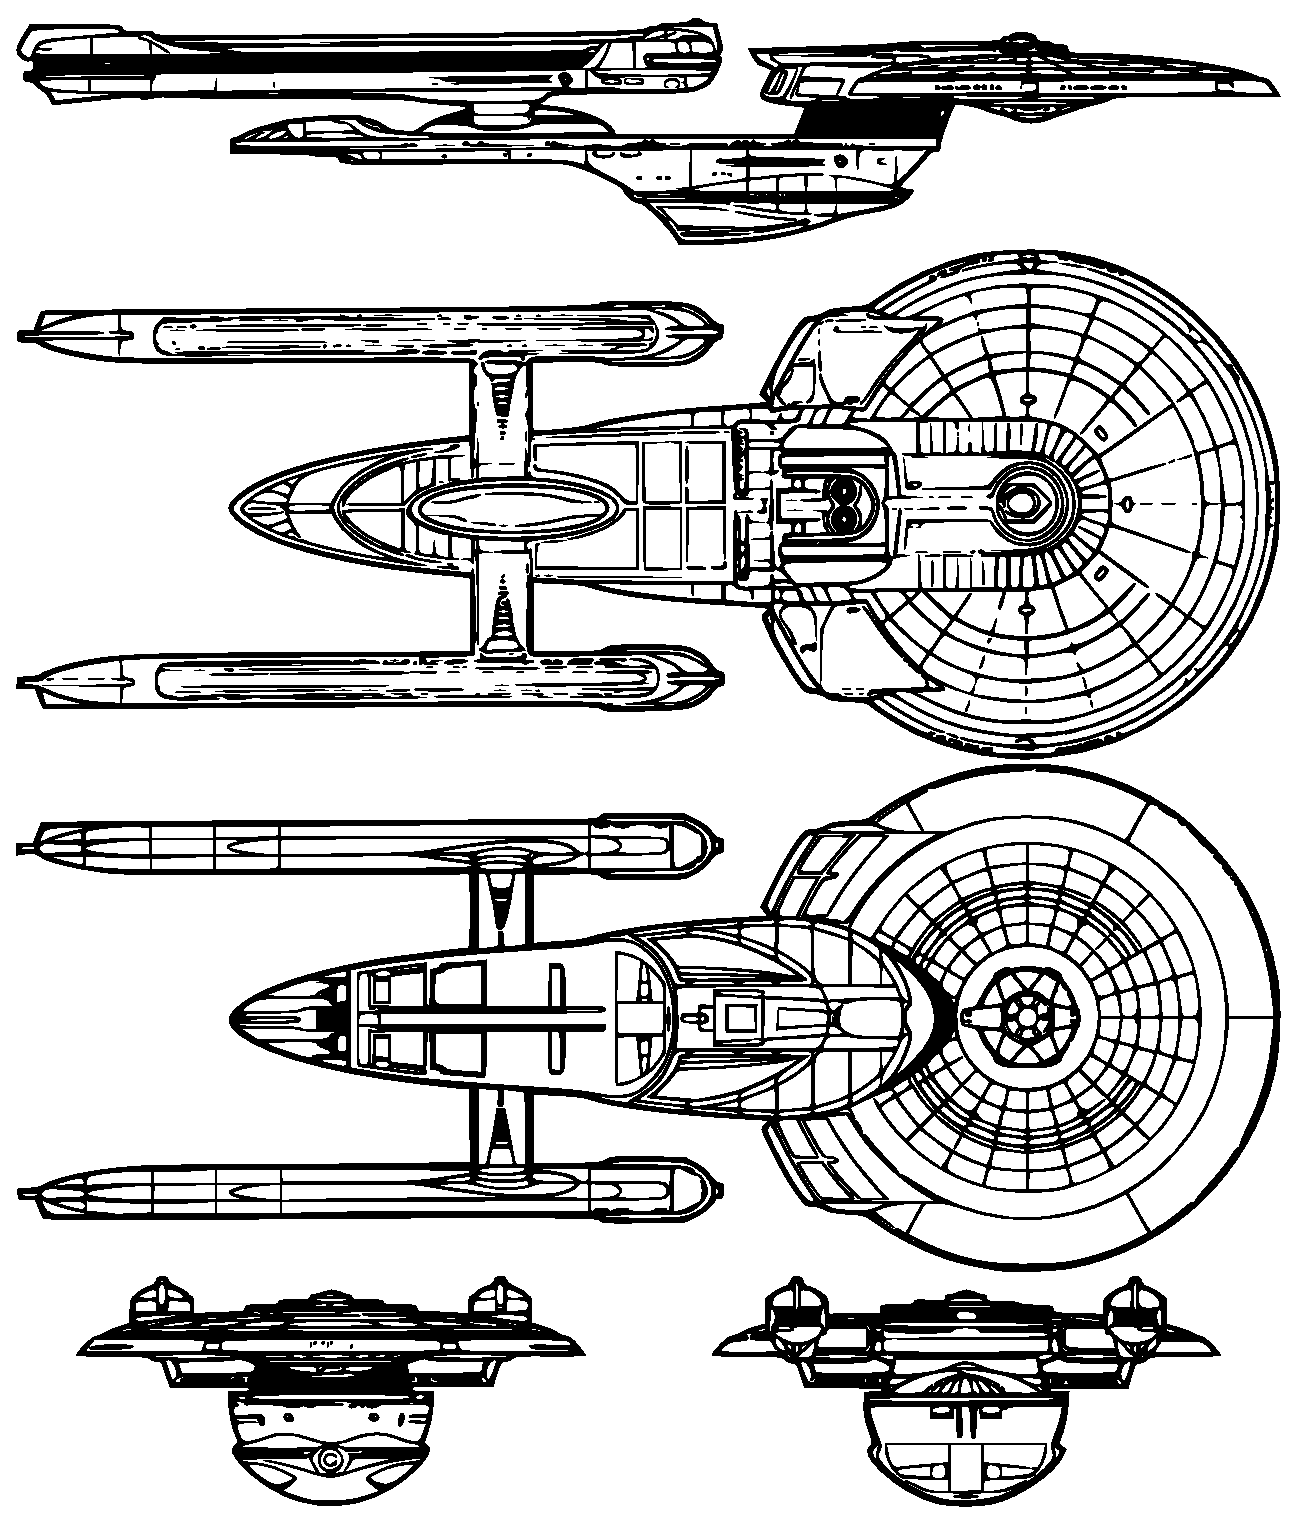
\includegraphics[width=0.8\linewidth]{img/ExcelsiorRefit.eps}\\
    \vspace{2ex}
    \footnotesize Overview of an \Class{Excelsior} starship
    \vspace{-2em}
\end{wrapfigure}

Finally, the Ferengi Alliance cannot really be called an ally nor an enemy ---
at any point they are whichever is more profitable. The Ferengi are a very
independent species, and small groups of Ferengi have spread throughout the
galaxy. It is not uncommon to come across Ferengi traders in any inhabited
region of space. Ferengi pirates have been known to attack and board Federation
ships, but these are usually isolated incidents.

\section{The Ship}

Your character will be serving aboard a newly-comissioned \Class{Excelsior}
starship, the same as the \Ship{USS Enterprise\-/B}. It features the usual
layout with saucer section, engineering section, and warp nacelle, but the
overall layout is more streamlined than the old \Class{Constitution}.

The ship is powered by a standard matter-antimatter warp drive. It is capable
of reaching warp nine, about 1500 times the speed of light. Standard cruising
speed is warp six, about 400 times the speed of light. The ship features an
experimental new dilithium recrystalization technology: the theta-matrix
compositor. This allows the ship to reuse the same dilithium crystals several
times before they need to be replaced.

\Class{Excelsior} ships have thirty-four decks, with deck one being the bridge.
The ship has the capacity to separate the saucer section from the engineering
section in times of emergency, with a battle bridge on deck nineteen. The
saucer section houses the impulse engines.

The ship phasers are standard dual-emitter type eight phasers. The ship has
five emitters on the forward saucer section, and one on the aft of the saucer.
There are also emitters positioned laterally port and starboard and an emitter
between the nacelles. Each emitter fires two beams. There are two primary
photon torpedo launchers in the forward section, and two more lower down the
neck. Aft launchers are located above the main shuttlebay.

For defence, the ship is equipped with deflector shields, which contain six
sections: forward, starboard, port, aft, dorsal, and ventral. The shields take
several seconds to come online, so surprise attacks can be devastating. The
shield frequency must be matched to that of your phasers in order to fire
through them, but if an enemy can match their phaser frequency to your shields
they can fire through them as well. Randomizing shield frequency can be an
effective defence against this. It is not yet possible to transport through
shields.

\section{Stardates}

Keeping track of date and time is no easy task when there are thousands of
planets involved and ships cause time-dilation as a standard practice. Soon
after it was founded, the Federation developed stardates for timekeeping.
Starfleet requires the use of stardates for all official records and logs. The
old Gregorian calendar is still sometimes used by Humans to refer to dates in
the distant past, or more rarely for personal use, but most people use
stardates even for day-to-day affairs.

Calculating the stardate is unfortunately complicated, because the series and
movies do not agree on any sort of scale or continuity. We will be using the
fan-based explanation provided by the \emph{Stardates in Star Trek
FAQ}\footnote{\emph{Stardates in Star Trek FAQ:}
\url{http://starchive.cs.umanitoba.ca/?stardates/}}, specifically the
conjectural history detailed in Part IV.

The current full stardate is [20]3574.5, which corresponds to approximately
February 20, 2315 on Earth. Each day is 0.5 units. The 20 is written in
brackets because it is not actually part of the stardate, but rather the
\emph{issue number}. Stardates reset to 0000 after 9999 and the next issue of
stardates begins.

\section{Conclusion}

I hope this document has answered many of your questions about the campaign
setting. Keep in mind that it serves only to inform and spark your imagination.
Please feel free to make things up and fill in details --- it's ok if they
don't quite jive with canon. While we are roleplaying, the Rule of Cool always
trumps because the main goal is to have fun.

\end{document}

